\documentclass[twoside]{book}

% Packages required by doxygen
\usepackage{fixltx2e}
\usepackage{calc}
\usepackage{doxygen}
\usepackage[export]{adjustbox} % also loads graphicx
\usepackage{graphicx}
\usepackage[utf8]{inputenc}
\usepackage{makeidx}
\usepackage{multicol}
\usepackage{multirow}
\PassOptionsToPackage{warn}{textcomp}
\usepackage{textcomp}
\usepackage[nointegrals]{wasysym}
\usepackage[table]{xcolor}

% NLS support packages
\usepackage[T2A]{fontenc}
\usepackage[ukrainian]{babel}

% Font selection
\usepackage[T1]{fontenc}
\usepackage[scaled=.90]{helvet}
\usepackage{courier}
\usepackage{amssymb}
\usepackage{sectsty}
\renewcommand{\familydefault}{\sfdefault}
\allsectionsfont{%
  \fontseries{bc}\selectfont%
  \color{darkgray}%
}
\renewcommand{\DoxyLabelFont}{%
  \fontseries{bc}\selectfont%
  \color{darkgray}%
}
\newcommand{\+}{\discretionary{\mbox{\scriptsize$\hookleftarrow$}}{}{}}

% Page & text layout
\usepackage{geometry}
\geometry{%
  a4paper,%
  top=2.5cm,%
  bottom=2.5cm,%
  left=2.5cm,%
  right=2.5cm%
}
\tolerance=750
\hfuzz=15pt
\hbadness=750
\setlength{\emergencystretch}{15pt}
\setlength{\parindent}{0cm}
\setlength{\parskip}{3ex plus 2ex minus 2ex}
\makeatletter
\renewcommand{\paragraph}{%
  \@startsection{paragraph}{4}{0ex}{-1.0ex}{1.0ex}{%
    \normalfont\normalsize\bfseries\SS@parafont%
  }%
}
\renewcommand{\subparagraph}{%
  \@startsection{subparagraph}{5}{0ex}{-1.0ex}{1.0ex}{%
    \normalfont\normalsize\bfseries\SS@subparafont%
  }%
}
\makeatother

% Headers & footers
\usepackage{fancyhdr}
\pagestyle{fancyplain}
\fancyhead[LE]{\fancyplain{}{\bfseries\thepage}}
\fancyhead[CE]{\fancyplain{}{}}
\fancyhead[RE]{\fancyplain{}{\bfseries\leftmark}}
\fancyhead[LO]{\fancyplain{}{\bfseries\rightmark}}
\fancyhead[CO]{\fancyplain{}{}}
\fancyhead[RO]{\fancyplain{}{\bfseries\thepage}}
\fancyfoot[LE]{\fancyplain{}{}}
\fancyfoot[CE]{\fancyplain{}{}}
\fancyfoot[RE]{\fancyplain{}{\bfseries\scriptsize Створено системою Doxygen }}
\fancyfoot[LO]{\fancyplain{}{\bfseries\scriptsize Створено системою Doxygen }}
\fancyfoot[CO]{\fancyplain{}{}}
\fancyfoot[RO]{\fancyplain{}{}}
\renewcommand{\footrulewidth}{0.4pt}
\renewcommand{\chaptermark}[1]{%
  \markboth{#1}{}%
}
\renewcommand{\sectionmark}[1]{%
  \markright{\thesection\ #1}%
}

% Indices & bibliography
\usepackage{natbib}
\usepackage[titles]{tocloft}
\setcounter{tocdepth}{3}
\setcounter{secnumdepth}{5}
\makeindex

% Hyperlinks (required, but should be loaded last)
\usepackage{ifpdf}
\ifpdf
  \usepackage[pdftex,pagebackref=true]{hyperref}
\else
  \usepackage[ps2pdf,pagebackref=true]{hyperref}
\fi
\hypersetup{%
  colorlinks=true,%
  linkcolor=blue,%
  citecolor=blue,%
  unicode%
}

% Custom commands
\newcommand{\clearemptydoublepage}{%
  \newpage{\pagestyle{empty}\cleardoublepage}%
}

\usepackage{caption}
\captionsetup{labelsep=space,justification=centering,font={bf},singlelinecheck=off,skip=4pt,position=top}

%===== C O N T E N T S =====

\begin{document}

% Titlepage & ToC
\hypersetup{pageanchor=false,
             bookmarksnumbered=true,
             pdfencoding=unicode
            }
\pagenumbering{alph}
\begin{titlepage}
\vspace*{7cm}
\begin{center}%
{\Large My Project \\[1ex]\large 333333 }\\
\vspace*{1cm}
{\large Створено системою Doxygen 1.8.13}\\
\end{center}
\end{titlepage}
\clearemptydoublepage
\pagenumbering{roman}
\tableofcontents
\clearemptydoublepage
\pagenumbering{arabic}
\hypersetup{pageanchor=true}

%--- Begin generated contents ---
\chapter{Алфавітний покажчик класів}
\section{Класи}
Класи, структури, об\textquotesingle{}єднання та інтерфейси з коротким описом.\begin{DoxyCompactList}
\item\contentsline{section}{\hyperlink{classmodAlphaCipher}{mod\+Alpha\+Cipher} \\*Шифрование методом Гронсфельда }{\pageref{classmodAlphaCipher}}{}
\end{DoxyCompactList}

\chapter{Покажчик файлв}
\section{Файли}
Повний список файлів.\begin{DoxyCompactList}
\item\contentsline{section}{\hyperlink{main_8cpp}{main.\+cpp} \\*Заголовочный файл для модуля \hyperlink{main_8cpp}{main.\+cpp} }{\pageref{main_8cpp}}{}
\item\contentsline{section}{\hyperlink{modAlphaCipher_8cpp}{mod\+Alpha\+Cipher.\+cpp} \\*Заголовочный файл для модуля \hyperlink{modAlphaCipher_8cpp}{mod\+Alpha\+Cipher.\+cpp} }{\pageref{modAlphaCipher_8cpp}}{}
\item\contentsline{section}{\hyperlink{modAlphaCipher_8h}{mod\+Alpha\+Cipher.\+h} \\*Заголовочный файл для модуля \hyperlink{modAlphaCipher_8h}{mod\+Alpha\+Cipher.\+h} }{\pageref{modAlphaCipher_8h}}{}
\end{DoxyCompactList}

\chapter{Класи}
\hypertarget{classmodAlphaCipher}{}\section{Клас mod\+Alpha\+Cipher}
\label{classmodAlphaCipher}\index{mod\+Alpha\+Cipher@{mod\+Alpha\+Cipher}}


Шифрование методом Гронсфельда  




{\ttfamily \#include $<$mod\+Alpha\+Cipher.\+h$>$}

\subsection*{Загальнодоступні елементи}
\begin{DoxyCompactItemize}
\item 
\hyperlink{classmodAlphaCipher_a4f0a86c20f5d836f66cb1e640d875e6b}{mod\+Alpha\+Cipher} ()=delete
\begin{DoxyCompactList}\small\item\em Валидация зашифрованного текста \end{DoxyCompactList}\item 
\hyperlink{classmodAlphaCipher_a6c6305969b8a57ac1c1c9cc5f5215b6d}{mod\+Alpha\+Cipher} (const string \&skey)
\begin{DoxyCompactList}\small\item\em Конструктор для установки ключа \end{DoxyCompactList}\item 
string \hyperlink{classmodAlphaCipher_a704e2999580f33b8c01ad634a3efb4dd}{encrypt} (const string \&open\+\_\+text)
\begin{DoxyCompactList}\small\item\em Зашифровывание \end{DoxyCompactList}\item 
string \hyperlink{classmodAlphaCipher_ad79b06b2d0df98964b9d86283adf9513}{decrypt} (const string \&cipher\+\_\+text)
\begin{DoxyCompactList}\small\item\em Расшифровывание \end{DoxyCompactList}\end{DoxyCompactItemize}
\subsection*{Приватні елементи}
\begin{DoxyCompactItemize}
\item 
vector$<$ int $>$ \hyperlink{classmodAlphaCipher_ad08ba0004ee53526e9110ff20daffb90}{convert} (const wstring \&ws)
\begin{DoxyCompactList}\small\item\em Преобразование строка-\/вектор \end{DoxyCompactList}\item 
string \hyperlink{classmodAlphaCipher_a0c204ef4200fbdd11e2e7f8a3018b396}{convert} (const vector$<$ int $>$ \&v)
\begin{DoxyCompactList}\small\item\em Преобразование вектор-\/строка \end{DoxyCompactList}\item 
wstring \hyperlink{classmodAlphaCipher_abe2b4d4ac6d40a1e1fec64953f047594}{towstr} (const string \&s)
\begin{DoxyCompactList}\small\item\em Валидация ключа \end{DoxyCompactList}\item 
string \hyperlink{classmodAlphaCipher_ac5726e023a298cccbdd65ceb4f0e705f}{fromwstr} (const wstring \&ws)
\begin{DoxyCompactList}\small\item\em Валидация открытого текста 4. \end{DoxyCompactList}\end{DoxyCompactItemize}
\subsection*{Приватні дані}
\begin{DoxyCompactItemize}
\item 
wstring \hyperlink{classmodAlphaCipher_a9f83731ae4d58df14e1df3bd089d7501}{num\+Alpha} = L\char`\"{}АБВГДЕЁЖЗИЙКЛМНОПРСТУФХЦЧШЩЪЫЬЭЮЯ\char`\"{}
\begin{DoxyCompactList}\small\item\em Русский алфавит попорядку \end{DoxyCompactList}\item 
map$<$ wchar\+\_\+t, int $>$ \hyperlink{classmodAlphaCipher_a9f0ca70558be9e08474f544aeaac55d8}{alpha\+Num}
\begin{DoxyCompactList}\small\item\em Ассоциативный массив\char`\"{}номер по символу\char`\"{}. \end{DoxyCompactList}\item 
vector$<$ int $>$ \hyperlink{classmodAlphaCipher_a318efb0cdcd8bc0c084097e175c2006b}{key}
\begin{DoxyCompactList}\small\item\em Ключ \end{DoxyCompactList}\end{DoxyCompactItemize}


\subsection{Детальний опис}
Шифрование методом Гронсфельда 

Ключ устанавливается в конструкторе.\+Для зашифровывания и расшифровывания предназначены методы encrypt и decrypt. \begin{DoxyWarning}{Застереження}
Реализация только для русского языка 
\end{DoxyWarning}


\subsection{Конструктор(и)}
\mbox{\Hypertarget{classmodAlphaCipher_a4f0a86c20f5d836f66cb1e640d875e6b}\label{classmodAlphaCipher_a4f0a86c20f5d836f66cb1e640d875e6b}} 
\index{mod\+Alpha\+Cipher@{mod\+Alpha\+Cipher}!mod\+Alpha\+Cipher@{mod\+Alpha\+Cipher}}
\index{mod\+Alpha\+Cipher@{mod\+Alpha\+Cipher}!mod\+Alpha\+Cipher@{mod\+Alpha\+Cipher}}
\subsubsection{\texorpdfstring{mod\+Alpha\+Cipher()}{modAlphaCipher()}\hspace{0.1cm}{\footnotesize\ttfamily [1/2]}}
{\footnotesize\ttfamily mod\+Alpha\+Cipher\+::mod\+Alpha\+Cipher (\begin{DoxyParamCaption}{ }\end{DoxyParamCaption})\hspace{0.3cm}{\ttfamily [delete]}}



Валидация зашифрованного текста 


\begin{DoxyParams}[1]{Аргументи}
\mbox{\tt in}  & {\em ws} & Зашифрованный текст в кодировке U\+T\+F-\/32. Не должен быть пустой строкой. Не должен содержать строчные символы и небуквы. \\
\hline
\end{DoxyParams}
\begin{DoxyReturn}{Повертає}
Валидный зашифрованный текст в кодировке U\+T\+F-\/32 
\end{DoxyReturn}

\begin{DoxyExceptions}{Обробка виняткових ситуацій}
{\em cipher\+\_\+error} & текст пустой или содержит недопустимые символы Конструктор без параметров\\
\hline
\end{DoxyExceptions}
Запрещен \mbox{\Hypertarget{classmodAlphaCipher_a6c6305969b8a57ac1c1c9cc5f5215b6d}\label{classmodAlphaCipher_a6c6305969b8a57ac1c1c9cc5f5215b6d}} 
\index{mod\+Alpha\+Cipher@{mod\+Alpha\+Cipher}!mod\+Alpha\+Cipher@{mod\+Alpha\+Cipher}}
\index{mod\+Alpha\+Cipher@{mod\+Alpha\+Cipher}!mod\+Alpha\+Cipher@{mod\+Alpha\+Cipher}}
\subsubsection{\texorpdfstring{mod\+Alpha\+Cipher()}{modAlphaCipher()}\hspace{0.1cm}{\footnotesize\ttfamily [2/2]}}
{\footnotesize\ttfamily mod\+Alpha\+Cipher\+::mod\+Alpha\+Cipher (\begin{DoxyParamCaption}\item[{const string \&}]{skey }\end{DoxyParamCaption})}



Конструктор для установки ключа 

Ключ проверяется на валидность. Переводится в кодировку U\+T\+F-\/32. Формируется вектор-\/ключ. 
\begin{DoxyParams}[1]{Аргументи}
\mbox{\tt in}  & {\em skey} & Ключ в кодировке U\+T\+F-\/8 \\
\hline
\end{DoxyParams}

\begin{DoxyExceptions}{Обробка виняткових ситуацій}
{\em cipher\+\_\+error} & ключ вырожденный \\
\hline
\end{DoxyExceptions}


\subsection{Опис методів компонент}
\mbox{\Hypertarget{classmodAlphaCipher_ad08ba0004ee53526e9110ff20daffb90}\label{classmodAlphaCipher_ad08ba0004ee53526e9110ff20daffb90}} 
\index{mod\+Alpha\+Cipher@{mod\+Alpha\+Cipher}!convert@{convert}}
\index{convert@{convert}!mod\+Alpha\+Cipher@{mod\+Alpha\+Cipher}}
\subsubsection{\texorpdfstring{convert()}{convert()}\hspace{0.1cm}{\footnotesize\ttfamily [1/2]}}
{\footnotesize\ttfamily vector$<$int$>$ mod\+Alpha\+Cipher\+::convert (\begin{DoxyParamCaption}\item[{const wstring \&}]{ws }\end{DoxyParamCaption})\hspace{0.3cm}{\ttfamily [private]}}



Преобразование строка-\/вектор 


\begin{DoxyParams}[1]{Аргументи}
\mbox{\tt in}  & {\em ws} & Строка в кодировке U\+T\+F-\/32 \\
\hline
\end{DoxyParams}
\begin{DoxyReturn}{Повертає}
Целочисленный вектор 
\end{DoxyReturn}
\mbox{\Hypertarget{classmodAlphaCipher_a0c204ef4200fbdd11e2e7f8a3018b396}\label{classmodAlphaCipher_a0c204ef4200fbdd11e2e7f8a3018b396}} 
\index{mod\+Alpha\+Cipher@{mod\+Alpha\+Cipher}!convert@{convert}}
\index{convert@{convert}!mod\+Alpha\+Cipher@{mod\+Alpha\+Cipher}}
\subsubsection{\texorpdfstring{convert()}{convert()}\hspace{0.1cm}{\footnotesize\ttfamily [2/2]}}
{\footnotesize\ttfamily string mod\+Alpha\+Cipher\+::convert (\begin{DoxyParamCaption}\item[{const vector$<$ int $>$ \&}]{v }\end{DoxyParamCaption})\hspace{0.3cm}{\ttfamily [private]}}



Преобразование вектор-\/строка 


\begin{DoxyParams}[1]{Аргументи}
\mbox{\tt in}  & {\em v} & Целочисленный вектор \\
\hline
\end{DoxyParams}
\begin{DoxyReturn}{Повертає}
Строка в кодировке U\+T\+F-\/8 
\end{DoxyReturn}
\mbox{\Hypertarget{classmodAlphaCipher_ad79b06b2d0df98964b9d86283adf9513}\label{classmodAlphaCipher_ad79b06b2d0df98964b9d86283adf9513}} 
\index{mod\+Alpha\+Cipher@{mod\+Alpha\+Cipher}!decrypt@{decrypt}}
\index{decrypt@{decrypt}!mod\+Alpha\+Cipher@{mod\+Alpha\+Cipher}}
\subsubsection{\texorpdfstring{decrypt()}{decrypt()}}
{\footnotesize\ttfamily std\+::string mod\+Alpha\+Cipher\+::decrypt (\begin{DoxyParamCaption}\item[{const string \&}]{cipher\+\_\+text }\end{DoxyParamCaption})}



Расшифровывание 


\begin{DoxyParams}[1]{Аргументи}
\mbox{\tt in}  & {\em cipher\+\_\+text} & Зашифрованный текст в кодировке U\+T\+F-\/8. Не должен быть пустой строкой. Не должен содержать строчные символы и небуквы. \\
\hline
\end{DoxyParams}
\begin{DoxyReturn}{Повертає}
Расифрованная строка в кодировке U\+T\+F-\/8 
\end{DoxyReturn}

\begin{DoxyExceptions}{Обробка виняткових ситуацій}
{\em cipher\+\_\+error} & текст пустой\\
\hline
\end{DoxyExceptions}
/$\ast$$\ast$ 
\begin{DoxyParams}[1]{Аргументи}
\mbox{\tt in}  & {\em cipher\+\_\+text} & Зашифрованный текст в кодировке U\+T\+F-\/8. Не должен быть пустой строкой. Не должен содержать строчные символы и небуквы. \\
\hline
\end{DoxyParams}
\begin{DoxyReturn}{Повертає}
Расифрованная строка в кодировке U\+T\+F-\/8 
\end{DoxyReturn}

\begin{DoxyExceptions}{Обробка виняткових ситуацій}
{\em cipher\+\_\+error} & текст пустой \\
\hline
\end{DoxyExceptions}
\mbox{\Hypertarget{classmodAlphaCipher_a704e2999580f33b8c01ad634a3efb4dd}\label{classmodAlphaCipher_a704e2999580f33b8c01ad634a3efb4dd}} 
\index{mod\+Alpha\+Cipher@{mod\+Alpha\+Cipher}!encrypt@{encrypt}}
\index{encrypt@{encrypt}!mod\+Alpha\+Cipher@{mod\+Alpha\+Cipher}}
\subsubsection{\texorpdfstring{encrypt()}{encrypt()}}
{\footnotesize\ttfamily std\+::string mod\+Alpha\+Cipher\+::encrypt (\begin{DoxyParamCaption}\item[{const string \&}]{open\+\_\+text }\end{DoxyParamCaption})}



Зашифровывание 


\begin{DoxyParams}[1]{Аргументи}
\mbox{\tt in}  & {\em open\+\_\+text} & Открытый текст в кодировке U\+T\+F-\/8. Не должен быть пустой строкой. Строчные символы автоматически преобразуются к прописным.\+Все не-\/буквы удаляются. \\
\hline
\end{DoxyParams}
\begin{DoxyReturn}{Повертає}
Зашифрованная строка в кодировке U\+T\+F-\/8 
\end{DoxyReturn}

\begin{DoxyExceptions}{Обробка виняткових ситуацій}
{\em cipher\+\_\+error} & текст пустой\\
\hline
\end{DoxyExceptions}

\begin{DoxyParams}[1]{Аргументи}
\mbox{\tt in}  & {\em open\+\_\+text} & Открытый текст. Не должен быть пустой строкой. Строчные символы автоматически преобразуются к прописным. Все не-\/буквы удаляются \\
\hline
\end{DoxyParams}
\begin{DoxyReturn}{Повертає}
Зашифрованная строка 
\end{DoxyReturn}

\begin{DoxyExceptions}{Обробка виняткових ситуацій}
{\em cipher\+\_\+error,если} & текст пустой \\
\hline
\end{DoxyExceptions}
\mbox{\Hypertarget{classmodAlphaCipher_ac5726e023a298cccbdd65ceb4f0e705f}\label{classmodAlphaCipher_ac5726e023a298cccbdd65ceb4f0e705f}} 
\index{mod\+Alpha\+Cipher@{mod\+Alpha\+Cipher}!fromwstr@{fromwstr}}
\index{fromwstr@{fromwstr}!mod\+Alpha\+Cipher@{mod\+Alpha\+Cipher}}
\subsubsection{\texorpdfstring{fromwstr()}{fromwstr()}}
{\footnotesize\ttfamily std\+::string mod\+Alpha\+Cipher\+::fromwstr (\begin{DoxyParamCaption}\item[{const wstring \&}]{ws }\end{DoxyParamCaption})\hspace{0.3cm}{\ttfamily [private]}}



Валидация открытого текста 4. 


\begin{DoxyParams}[1]{Аргументи}
\mbox{\tt in}  & {\em ws} & Открытый текст в кодировке U\+T\+F32. Не должен быть пустой строкой. Строчные символы автоматически преобразуются к прописным. \\
\hline
\end{DoxyParams}
\begin{DoxyReturn}{Повертає}
Валидный открытый текст в кодировке U\+T\+F-\/32 
\end{DoxyReturn}

\begin{DoxyExceptions}{Обробка виняткових ситуацій}
{\em cipher\+\_\+error} & текст пустой или содержит недопустимые символы \\
\hline
\end{DoxyExceptions}
\mbox{\Hypertarget{classmodAlphaCipher_abe2b4d4ac6d40a1e1fec64953f047594}\label{classmodAlphaCipher_abe2b4d4ac6d40a1e1fec64953f047594}} 
\index{mod\+Alpha\+Cipher@{mod\+Alpha\+Cipher}!towstr@{towstr}}
\index{towstr@{towstr}!mod\+Alpha\+Cipher@{mod\+Alpha\+Cipher}}
\subsubsection{\texorpdfstring{towstr()}{towstr()}}
{\footnotesize\ttfamily std\+::wstring mod\+Alpha\+Cipher\+::towstr (\begin{DoxyParamCaption}\item[{const string \&}]{s }\end{DoxyParamCaption})\hspace{0.3cm}{\ttfamily [private]}}



Валидация ключа 


\begin{DoxyParams}[1]{Аргументи}
\mbox{\tt in}  & {\em ws} & Ключ в кодировке U\+T\+F-\/32. Не должен быть пустой строкой. Строчные символы автоматически преобразуются к прописным. \\
\hline
\end{DoxyParams}
\begin{DoxyReturn}{Повертає}
Валидный ключ в кодировке U\+T\+F-\/32 
\end{DoxyReturn}

\begin{DoxyExceptions}{Обробка виняткових ситуацій}
{\em cipher\+\_\+error} & ключ пустой или содержит недопустимые символы \\
\hline
\end{DoxyExceptions}


\subsection{Компонентні дані}
\mbox{\Hypertarget{classmodAlphaCipher_a9f0ca70558be9e08474f544aeaac55d8}\label{classmodAlphaCipher_a9f0ca70558be9e08474f544aeaac55d8}} 
\index{mod\+Alpha\+Cipher@{mod\+Alpha\+Cipher}!alpha\+Num@{alpha\+Num}}
\index{alpha\+Num@{alpha\+Num}!mod\+Alpha\+Cipher@{mod\+Alpha\+Cipher}}
\subsubsection{\texorpdfstring{alpha\+Num}{alphaNum}}
{\footnotesize\ttfamily map$<$wchar\+\_\+t,int$>$ mod\+Alpha\+Cipher\+::alpha\+Num\hspace{0.3cm}{\ttfamily [private]}}



Ассоциативный массив\char`\"{}номер по символу\char`\"{}. 

\mbox{\Hypertarget{classmodAlphaCipher_a318efb0cdcd8bc0c084097e175c2006b}\label{classmodAlphaCipher_a318efb0cdcd8bc0c084097e175c2006b}} 
\index{mod\+Alpha\+Cipher@{mod\+Alpha\+Cipher}!key@{key}}
\index{key@{key}!mod\+Alpha\+Cipher@{mod\+Alpha\+Cipher}}
\subsubsection{\texorpdfstring{key}{key}}
{\footnotesize\ttfamily vector$<$int$>$ mod\+Alpha\+Cipher\+::key\hspace{0.3cm}{\ttfamily [private]}}



Ключ 

\mbox{\Hypertarget{classmodAlphaCipher_a9f83731ae4d58df14e1df3bd089d7501}\label{classmodAlphaCipher_a9f83731ae4d58df14e1df3bd089d7501}} 
\index{mod\+Alpha\+Cipher@{mod\+Alpha\+Cipher}!num\+Alpha@{num\+Alpha}}
\index{num\+Alpha@{num\+Alpha}!mod\+Alpha\+Cipher@{mod\+Alpha\+Cipher}}
\subsubsection{\texorpdfstring{num\+Alpha}{numAlpha}}
{\footnotesize\ttfamily wstring mod\+Alpha\+Cipher\+::num\+Alpha = L\char`\"{}АБВГДЕЁЖЗИЙКЛМНОПРСТУФХЦЧШЩЪЫЬЭЮЯ\char`\"{}\hspace{0.3cm}{\ttfamily [private]}}



Русский алфавит попорядку 



Документація цих класів була створена з файлів\+:\begin{DoxyCompactItemize}
\item 
\hyperlink{modAlphaCipher_8h}{mod\+Alpha\+Cipher.\+h}\item 
\hyperlink{modAlphaCipher_8cpp}{mod\+Alpha\+Cipher.\+cpp}\end{DoxyCompactItemize}

\chapter{Файли}
\hypertarget{main_8cpp}{}\section{Файл main.\+cpp}
\label{main_8cpp}\index{main.\+cpp@{main.\+cpp}}


Заголовочный файл для модуля \hyperlink{main_8cpp}{main.\+cpp}.  


{\ttfamily \#include $<$iostream$>$}\newline
{\ttfamily \#include $<$cctype$>$}\newline
{\ttfamily \#include $<$codecvt$>$}\newline
{\ttfamily \#include $<$locale$>$}\newline
{\ttfamily \#include \char`\"{}mod\+Alpha\+Cipher.\+h\char`\"{}}\newline
Діаграма включених заголовочних файлів для main.\+cpp\+:
\nopagebreak
\begin{figure}[H]
\begin{center}
\leavevmode
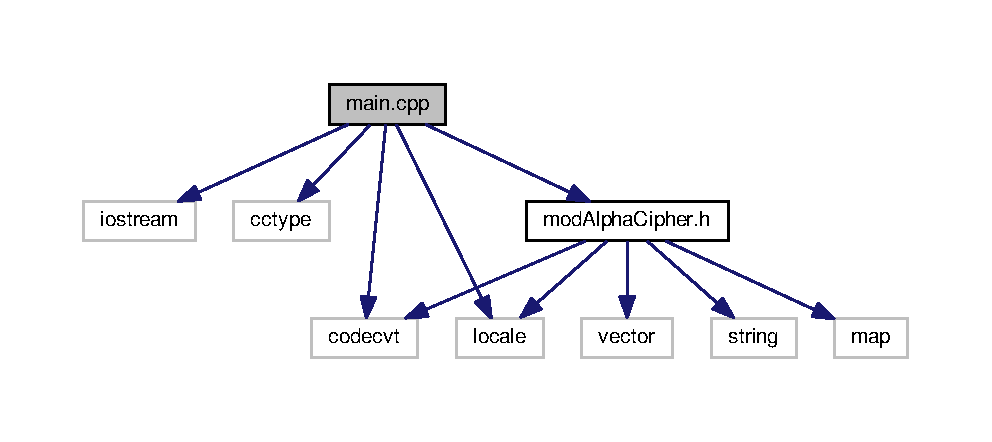
\includegraphics[width=350pt]{main_8cpp__incl}
\end{center}
\end{figure}
\subsection*{Функції}
\begin{DoxyCompactItemize}
\item 
bool \hyperlink{main_8cpp_a3eacb83174d2a9fbf9b313ebf1a9a883}{is\+Valid} (const string \&s)
\item 
int \hyperlink{main_8cpp_a3c04138a5bfe5d72780bb7e82a18e627}{main} (int argc, char $\ast$$\ast$argv)
\begin{DoxyCompactList}\small\item\em Интерфейс программы \end{DoxyCompactList}\end{DoxyCompactItemize}


\subsection{Детальний опис}
Заголовочный файл для модуля \hyperlink{main_8cpp}{main.\+cpp}. 

\begin{DoxyAuthor}{Автор}
Козин А.\+В. 
\end{DoxyAuthor}
\begin{DoxyVersion}{Версія}
1.\+0.\+0 
\end{DoxyVersion}
\begin{DoxyDate}{Дата}
13.\+06.\+2019 
\end{DoxyDate}


\subsection{Опис функцій}
\mbox{\Hypertarget{main_8cpp_a3eacb83174d2a9fbf9b313ebf1a9a883}\label{main_8cpp_a3eacb83174d2a9fbf9b313ebf1a9a883}} 
\index{main.\+cpp@{main.\+cpp}!is\+Valid@{is\+Valid}}
\index{is\+Valid@{is\+Valid}!main.\+cpp@{main.\+cpp}}
\subsubsection{\texorpdfstring{is\+Valid()}{isValid()}}
{\footnotesize\ttfamily bool is\+Valid (\begin{DoxyParamCaption}\item[{const string \&}]{s }\end{DoxyParamCaption})}

\mbox{\Hypertarget{main_8cpp_a3c04138a5bfe5d72780bb7e82a18e627}\label{main_8cpp_a3c04138a5bfe5d72780bb7e82a18e627}} 
\index{main.\+cpp@{main.\+cpp}!main@{main}}
\index{main@{main}!main.\+cpp@{main.\+cpp}}
\subsubsection{\texorpdfstring{main()}{main()}}
{\footnotesize\ttfamily int main (\begin{DoxyParamCaption}\item[{int}]{argc,  }\item[{char $\ast$$\ast$}]{argv }\end{DoxyParamCaption})}



Интерфейс программы 

Осуществелние выбора ключа и операции 0, 1 или 2. В зависимости от выбора выполняются следующие действия\+: выход, зашифровка, расшифровка. ввод ключа

ввод числа 
\hypertarget{modAlphaCipher_8cpp}{}\section{Файл mod\+Alpha\+Cipher.\+cpp}
\label{modAlphaCipher_8cpp}\index{mod\+Alpha\+Cipher.\+cpp@{mod\+Alpha\+Cipher.\+cpp}}


Заголовочный файл для модуля \hyperlink{modAlphaCipher_8cpp}{mod\+Alpha\+Cipher.\+cpp}.  


{\ttfamily \#include \char`\"{}mod\+Alpha\+Cipher.\+h\char`\"{}}\newline
Діаграма включених заголовочних файлів для mod\+Alpha\+Cipher.\+cpp\+:
\nopagebreak
\begin{figure}[H]
\begin{center}
\leavevmode
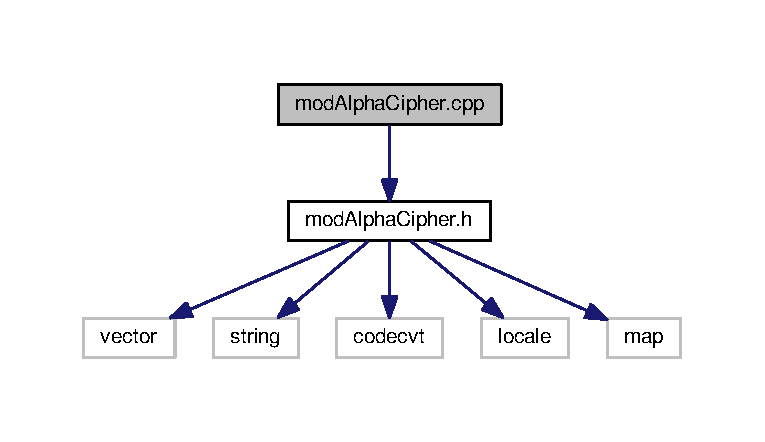
\includegraphics[width=350pt]{modAlphaCipher_8cpp__incl}
\end{center}
\end{figure}


\subsection{Детальний опис}
Заголовочный файл для модуля \hyperlink{modAlphaCipher_8cpp}{mod\+Alpha\+Cipher.\+cpp}. 

\begin{DoxyAuthor}{Автор}
Максимов О.\+В. 
\end{DoxyAuthor}
\begin{DoxyVersion}{Версія}
1.\+0.\+0 
\end{DoxyVersion}
\begin{DoxyDate}{Дата}
13.\+06.\+2019 
\end{DoxyDate}

\hypertarget{modAlphaCipher_8h}{}\section{Файл mod\+Alpha\+Cipher.\+h}
\label{modAlphaCipher_8h}\index{mod\+Alpha\+Cipher.\+h@{mod\+Alpha\+Cipher.\+h}}


Заголовочный файл для модуля \hyperlink{modAlphaCipher_8h}{mod\+Alpha\+Cipher.\+h}.  


{\ttfamily \#include $<$vector$>$}\newline
{\ttfamily \#include $<$string$>$}\newline
{\ttfamily \#include $<$codecvt$>$}\newline
{\ttfamily \#include $<$locale$>$}\newline
{\ttfamily \#include $<$map$>$}\newline
Діаграма включених заголовочних файлів для mod\+Alpha\+Cipher.\+h\+:
\nopagebreak
\begin{figure}[H]
\begin{center}
\leavevmode
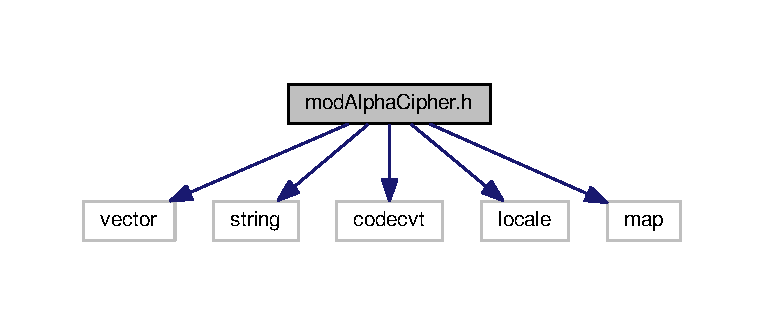
\includegraphics[width=350pt]{modAlphaCipher_8h__incl}
\end{center}
\end{figure}
Граф файлів, які включають цей файл\+:
\nopagebreak
\begin{figure}[H]
\begin{center}
\leavevmode
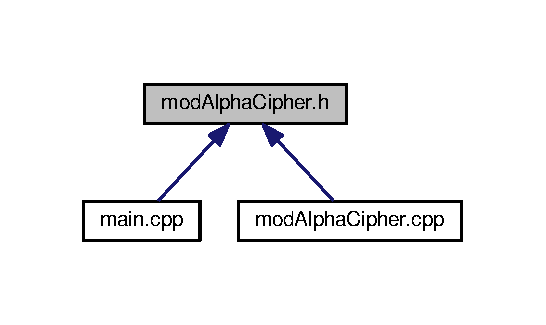
\includegraphics[width=262pt]{modAlphaCipher_8h__dep__incl}
\end{center}
\end{figure}
\subsection*{Класи}
\begin{DoxyCompactItemize}
\item 
class \hyperlink{classmodAlphaCipher}{mod\+Alpha\+Cipher}
\begin{DoxyCompactList}\small\item\em Шифрование методом Гронсфельда \end{DoxyCompactList}\end{DoxyCompactItemize}


\subsection{Детальний опис}
Заголовочный файл для модуля \hyperlink{modAlphaCipher_8h}{mod\+Alpha\+Cipher.\+h}. 

\begin{DoxyAuthor}{Автор}
Максимов О.\+В. 
\end{DoxyAuthor}
\begin{DoxyVersion}{Версія}
1.\+0.\+0 
\end{DoxyVersion}
\begin{DoxyDate}{Дата}
13.\+06.\+2019 
\end{DoxyDate}

%--- End generated contents ---

% Index
\backmatter
\newpage
\phantomsection
\clearemptydoublepage
\addcontentsline{toc}{chapter}{Предметний покажчик}
\printindex

\end{document}
